The final option for event definition is a user application. 
The user specifies the application name and the input file containing the specific input information 
needed by the application when it is running in the backend. 
As will be discussed later, when they use an additional application not provided, the user is also required 
to edit the tools registry file. There they must include a new event application with the same name 
and the location where that application can be found relative to the tools application directory. 
If running on DesignSafe, that application must be built and must be available on the Stampede2 supercomputer. 

Note: Given how DesignSafe runs the applications through Agave, the file permissions of this application must be 
world readable and executable (i.e., when a user runs their application through DesignSafe and Agave, they are not running it as themselves!)

\begin{figure}[!htbp]
  \centering {
    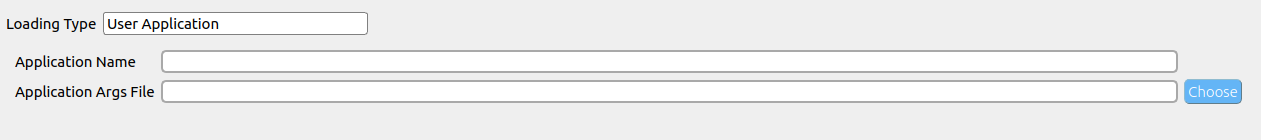
\includegraphics[width=1.0\textwidth]
    {usage/figures/userAppEvent.png} }
  \caption{User defined event}
  \label{fig:user_defined_event_panel}
\end{figure}
